\documentclass[]{article}
\usepackage{enumitem,amssymb,tikz,siunitx, pgfplots}
\usetikzlibrary{calc,matrix, arrows.meta, positioning, decorations,decorations.markings, math}
\newlist{todolist}{itemize}{2}
\setlist[todolist]{label=$\square$}
\usepackage{pifont}
\newcommand{\cmark}{\ding{51}}%
\newcommand{\xmark}{\ding{55}}%
\newcommand{\done}{\rlap{$\square$}{\raisebox{2pt}{\large\hspace{1pt}\cmark}}%
	\hspace{-2.5pt}}
\newcommand{\wontfix}{\rlap{$\square$}{\large\hspace{1pt}\xmark}}


\newcommand{\senods}[1]{
{#1}%
{%
	{0}{ 0.0000 }%
	{b}{now this is b}%
	{c}{you want me to do c?}%
}%
{[nada]}%
}


%opening
\title{Proyecto Assembler ARM Cortex M0+}
\author{Santiago Calligari, Gerónimo Nestares}
\begin{document}
\maketitle


\section*{Preambulo}
\textbf{\scriptsize{Bitacora. (1/6/2022)}}\\
Se nos presento la idea y oportunidad de crear un programa en el lenguaje ensamblador de la placa de desarrollo Raspberry Pi Pico. \\
Este proyecto cuenta como el proyecto final del cuatrimestre y este archivo, como el historial, conjunto con git de nuestra historia escribiendo el codigo y entendiendo ensamblador de ARM.	


\section*{Hoja de ruta}
Para generar senos contando pura y exclusivamente con ondas digitales podemos contar con dos formas, voy a proceder a comentar la primera, PWM o modulación por ancho de pulsos.


\section*{Modulación Por Ancho de Pulsos}
\textbf{\scriptsize{Voltajes Arbitrarios A Partir de Valores Fijos}}\\

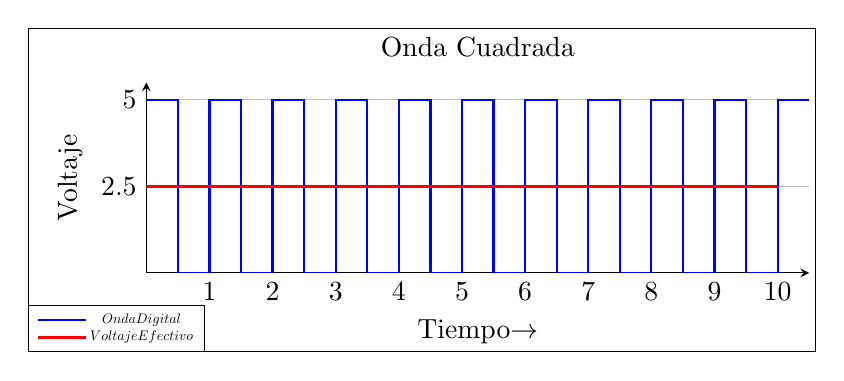
\begin{tikzpicture}
	\draw (-1.5,-1) -- (8.5,-1) -- (8.5,3.1) -- (-1.5,3.1) -- (-1.5,-1);
	\begin{axis}[
		legend style={nodes = {scale=0.5, transform shape}, at={(0.088,-0.17)}},
		legend entries={$Onda Digital$\\$Voltaje Efectivo$\\},
		ymajorgrids=true,
		width=10cm,
		height=4cm,
		x axis line style={-stealth},
		y axis line style={-stealth},
		title={Onda Cuadrada},
		ymax = 5.5,xmax=10.5,
		ymin = 0, xmin = 0,
		axis lines*=center,
		xtick distance=1,
		ytick={0,2.5,5},
		xlabel={Tiempo$\rightarrow$},
		ylabel={Voltaje},
		xlabel near ticks,
		ylabel near ticks]
		\addplot+[blue, thick, no marks ,const plot]
		coordinates{ 
			      (0,5) (0.5,5) (0.5,0)
			(1,0) (1,5) (1.5,5) (1.5,0)
			(2,0) (2,5) (2.5,5) (2.5,0)
			(3,0) (3,5) (3.5,5) (3.5,0)
			(4,0) (4,5) (4.5,5) (4.5,0)
			(5,0) (5,5) (5.5,5) (5.5,0)
			(6,0) (6,5) (6.5,5) (6.5,0)
			(7,0) (7,5) (7.5,5) (7.5,0)
			(8,0) (8,5) (8.5,5) (8.5,0)
			(9,0) (9,5) (9.5,5) (9.5,0)
			(10,0) (10,5) (10.5,5) 
		};
		\addplot+[red, very thick, no marks ,const plot]
		coordinates{(0,2.5) (10,2.5)};
\end{axis}
\end{tikzpicture}\\
Acá podemos ver una onda digital con un Ciclo de Trabajo de 50\%, lo que quiere decir que el 50\% de una unidad del tiempo esta prendido y lo restante apagado, esto, llevado a cabo millones de veces por segundo nos entrega un resultado llamado voltaje efectivo, el resultado de una onda con un Ciclo de Trabajo del 50\% y un Voltaje de 5 Voltios es un Voltaje Efectivo de 2.5 Voltios, como se puede observar en la figura inmediatamente superior.
\\Modificando el ciclo de trabajo de un procesador, podemos emular una onda analógica con bastante precisión. Ahora ¿Como pasamos de una onda plana a una onda Sinusoidal?. Viene al rescate la segunda sección.
\subsection*{Tabla de consulta}
El seno es una función periódica, con periodo T = $\frac{1}{F}$ = 2$\pi$ entonces podemos llegar a que no hay que calcular el seno con potencia del procesador cada vez que lo necesitamos, solamente nos fijamos en una tabla con un $\Delta$x particular. Una tabla de ejemplo sería ésta;
\begin{table}[h!]
	\begin{tabular}{|c|c|c|c|} 
		\hline
		 0.0000 & 0.3827 & 0.7071 & 0.9239 \\ \hline
	     1.0000 & 0.9239 & 0.7071 & 0.3827 \\ \hline
		 0.0000 &-0.3827 &-0.7071 &-0.9239 \\ \hline
		-1.0000 &-0.9239 &-0.7071 &-0.3827  \\\hline
	\end{tabular}
\end{table}\\
Lo que genera un seno de esta forma;\\
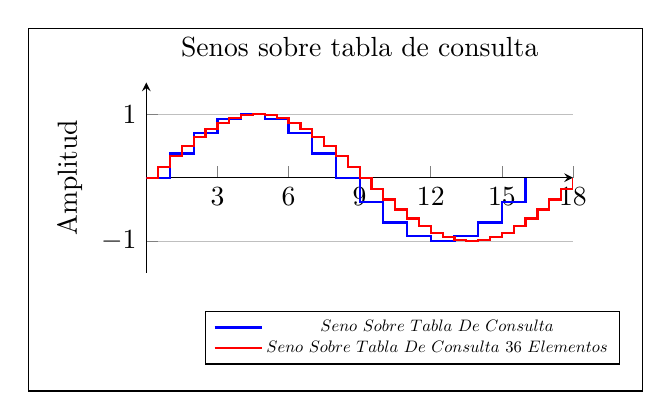
\begin{tikzpicture}
	\draw (-1.5,-1.5) -- (6.3,-1.5) -- (6.3,3.1) -- (-1.5,3.1) -- (-1.5,-1.5);
	\begin{axis}[
		legend style={nodes = {scale=0.6, transform shape}, at={(1.11,-0.2)}},
		legend entries={$Seno\ Sobre\ Tabla\ De\ Consulta$\\$Seno\ Sobre\ Tabla\ De\ Consulta\ 36\ Elementos$\\},
		ymajorgrids=true,
		width=7cm,
		height=4cm,
		x axis line style={-stealth},
		y axis line style={-stealth},
		title={Senos sobre tabla de consulta},
		ymax = 1.5,xmax=18,
		ymin = -1.5, xmin = 0,
		axis lines*=center,
		xtick distance=3,
		ytick={-1,0,1},
		ylabel={Amplitud},
		xlabel near ticks,
		ylabel near ticks]
		\addplot+[blue, thick, no marks, const plot]
		coordinates{
			( 0 , 0.0000 )( 1 , 0.3827 )( 2 , 0.7071 )( 3 , 0.9239 )( 4 , 1.0000 )( 5 , 0.9239 )( 6 , 0.7071 )( 7 , 0.3827 )( 8 , 0.0000 )( 9 , -0.3827 )( 10 , -0.7071 )( 11 , -0.9239 )( 12 , -1.0000 )( 13 , -0.9239 )( 14 , -0.7071 )( 15 , -0.3827)(16, 0)
		};
		\addplot+[red, thick, no marks, const plot]
		coordinates{(.0 , 0.0000 )( 0.5 , 0.1736 )( 1.0 , 0.3420 )( 1.5 , 0.5000 )( 2.0 , 0.6428 )( 2.5 , 0.7660 )( 3.0 , 0.8660 )( 3.5 , 0.9397 )( 4.0 , 0.9848 )( 4.5 , 1.0000 )( 5.0 , 0.9848 )( 5.5 , 0.9397 )( 6.0 , 0.8660 )( 6.5 , 0.7660 )( 7.0 , 0.6428 )( 7.5 , 0.5000 )( 8.0 , 0.3420 )( 8.5 , 0.1736 )( 9.0 , 0.0000 )( 9.5 , -0.1736 )( 10.0 , -0.3420 )( 10.5 , -0.5000 )( 11.0 , -0.6428 )( 11.5 , -0.7660 )( 12.0 , -0.8660 )( 12.5 , -0.9397 )( 13.0 , -0.9848 )( 13.5 , -1.0000 )( 14.0 , -0.9848 )( 14.5 , -0.9397 )( 15.0 , -0.8660 )( 15.5 , -0.7660 )( 16.0 , -0.6428 )( 16.5 , -0.5000 )( 17.0 , -0.3420 )( 17.5 , -0.1736 )(18, 0.0000)};
	\end{axis}
\end{tikzpicture}\\
Desde la gráfica de estas dos funciones podemos deducir que mientras más elementos tenga nuestras tablas de consulta mayor va a ser la precisión del seno.
Sabiendo el valor de los senos en un punto X podemos llegar a un valor de $D_{c}$ para poder generar una onda cuasi analógica.

\section*{El Principal Problema}
Nuestra placa de desarrollo, la RP2040 no cuenta con un F.P.U. debemos usar nuestro A.L.U. para simular coma flotante desde assembler debemos crear nuestro dato.
\end{document}
